\documentclass[a4paper]{article}
\usepackage{student}
\usepackage{hyperref}
\usepackage{graphicx}
\usepackage{algorithm}
\usepackage{algorithmic}
\usepackage{breqn}
\usepackage{subcaption}
\usepackage{multirow}
\usepackage{psfrag}
\usepackage{url}
\usepackage{hyperref}
%\usepackage[colorlinks]{hyperref}
\usepackage{cleveref}
\usepackage{booktabs}
\usepackage{rotating}
\usepackage{colortbl}
\usepackage{paralist}
%\usepackage{geometry}
\usepackage{epstopdf}
\usepackage{nag}
\usepackage{microtype}
\usepackage{siunitx}
\usepackage{nicefrac}
% for random text
\usepackage{lipsum}
\usepackage[english]{babel}
\usepackage[pangram]{blindtext}
% for tikz figures
\usepackage{listings}
\usepackage{tikz}
\usetikzlibrary{fit,positioning,arrows.meta,shapes,arrows}
% Metadata
\date{\today}
\setmodule{SIT742: Modern Data Science}
\setterm{Trimester 2, 2024}

%-------------------------------%
% Other details
% TODO: Fill these
%-------------------------------%
\title{Assignment 1}
\setmembername{SIT742}  % Fill group member names
%\setmemberuid{u1234567, u7654321}  % Fill group member uids (same order)

%-------------------------------%
% Add / Delete commands and packages
% TODO: Add / Delete here as you need
%-------------------------------%
\usepackage{amsmath,amssymb,bm}

\newcommand{\KL}{\mathrm{KL}}
\newcommand{\R}{\mathbb{R}}
\newcommand{\E}{\mathbb{E}}
\newcommand{\T}{\top}

\newcommand{\expdist}[2]{%
        \normalfont{\textsc{Exp}}(#1, #2)%
    }
\newcommand{\expparam}{\bm \lambda}
\newcommand{\Expparam}{\bm \Lambda}
\newcommand{\natparam}{\bm \eta}
\newcommand{\Natparam}{\bm H}
\newcommand{\sufstat}{\bm u}

% Main document
\begin{document}
    % Add header
    \header{}



    \begin{center}
        \fbox{\fbox{\parbox{5.5in}{\centering
\begin{description}
    \item [Extension Request] 
    Students with difficulty in meeting the deadline 
    because of various reasons,
    must apply for an assignment extension 
    no later than 8:00pm on 12/08/2024 (Monday).
    Apply via `\texttt{CloudDeakin}', 
    the menu item `\texttt{Extension Request}' 
    under the `\texttt{Assessment}' drop-down menu. 
    \item[\href{https://www.deakin.edu.au/students/studying/academic-integrity}{Academic Integrity}] 
    All assignment will be checked for plagiarism, 
    and any academic misconduct will be reported to 
    unit chair and university.

    \item[Generative AI] Deakin's Policy and advices on responsible usage of Generative AI in your studies: \url{https://www.deakin.edu.au/students/study-support/study-resources/artificial-intelligence}
\end{description} 
}}}
 
      \end{center}

      \section*{Instructions}


      \subsection*{Assignment Questions}\label{sec:question}
      
      There are total \textbf{2} parts in the assessment task:
      \begin{description}
      \item[Part $1$] 
      The first part will focus on the basic Python programming skills
      which includes the \texttt{data types}, the \texttt{control flow}, the \texttt{function},
      the \texttt{modules and library} from \href{https://github.com/tulip-lab/sit742/tree/develop/Jupyter/M02-Python}{\textbf{M02}}.
          
      \item[Part $2$] 
      The second part is for those who are aiming to 
      achieve `\texttt{High Distinction}' (HD) for this assessment task,
      and it will focus on more advanced Python programming skills for data science on particular scenario. 
      This part will require the knowledge covered in \href{https://github.com/tulip-lab/sit742/tree/develop/Jupyter/M02-Python}{\textbf{M02}} and also some part of the \href{https://github.com/tulip-lab/sit742/blob/develop/Jupyter/M03-BigData/M03D-DataAcquisition-I.ipynb}{\textbf{M03}}, 
      in particular, 
      \texttt{numpy} and beyond.
      \end{description}
      

    
\subsection*{What to Submit?}\label{sec:submit}

You are required to 
submit the following completed files to 
the corresponding \emph{Assignment} (Dropbox) in CloudDeakin:
\begin{description} 
\item[\texttt{SIT742Task1.ipynb}] 
The completed notebook with all the run-able code on all requirements.

In general, 
you need to complete, \textcolor{red}{\textbf{save}} the results of running, 
and submit your \textbf{notebook} 
from Python platform such as \texttt{Google Colab}. 
You need to clearly list the answer for each question,
and the expected format from your notebook will 
be like in~\Cref{fig:format}. 

\begin{figure}[H]
    \centering
    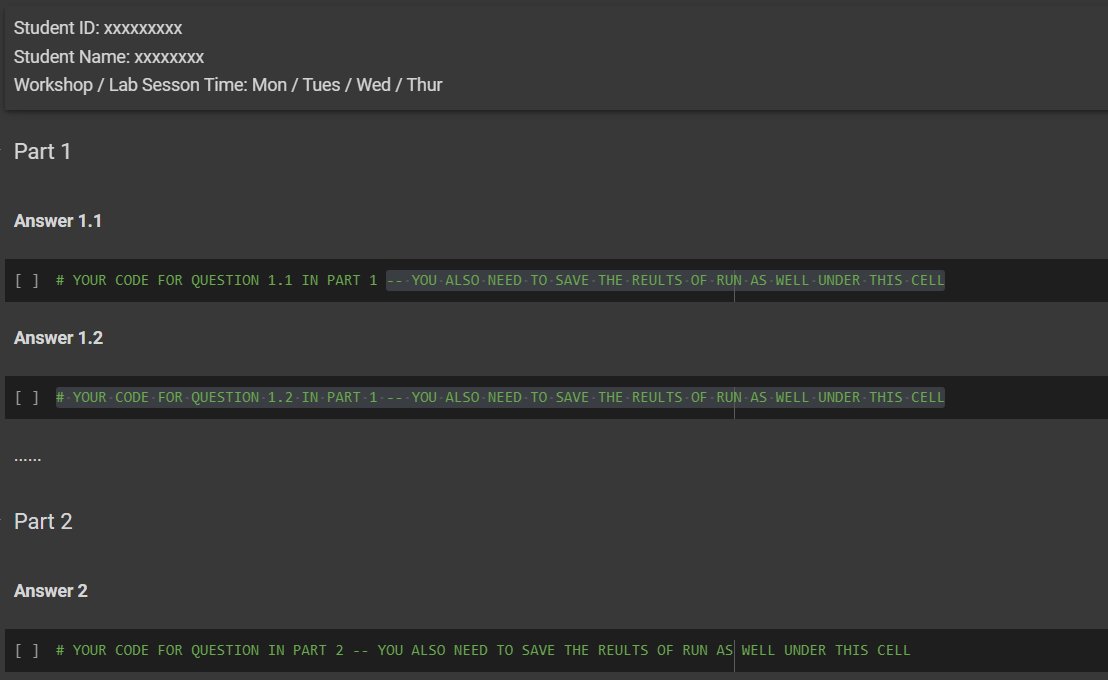
\includegraphics[width=0.8\columnwidth]{figure/assigment1.png}
    \caption{Notebook Format}
    \label{fig:format}
\end{figure}
    

\item[\texttt{SIT742Task1Part2.avi}] (Only if you choose to work on \emph{Part 2} of this assessment task)
A video demonstration between $5$ and $10$ minutes,
and the file format can be other common ones,
such as `\texttt{MKV}', `\texttt{WMV}', `\texttt{MOV}' etc. 

If you are aiming to achieve `\texttt{High Distinction}' (HD) and choose to work on \emph{Part 2} of this assessment task,
one important submission is a \textbf{short video} 
in which \emph{You} orally present the solutions 
that you provide in the notebook 
and illustrate the running of code line by line.

\item[\texttt{SIT742Task1Part2report.pdf}] (Only if you choose to work on \emph{Part 2} of this assessment task)
A short essay report with no more than 500 words,
and the file format can be other common ones,
such as `\texttt{.pdf}', `\texttt{.doc}', `\texttt{docx}' etc.

If you are aiming to achieve `\texttt{High Distinction}' (HD) and choose to work on \emph{Part 2} of this assessment task,
another important submission is a \textbf{short essay} 
in which \emph{You} will explain the code you wrote for the solution,
any of the resource or material which has been helpful 
to resolve the problem, 
and illustrate if there is any alternative way to solve the problem.
In addition, you will also need to follow the common essay writing structure which could be found in \url{https://www.deakin.edu.au/students/study-support/study-resources/academic-skills/essay-writing}

\end{description}

% present how you solve the part 2 questions,
%  and detail the .
%     Part 2 of the assignment has two choices,
%     for students who have the student ID on \textbf{odd} number, 
%     you will need to do the first choice,
%     and for students who have the student ID on \textbf{even} number,
%     you will need to do the second choice.
%     \textcolor{red}{If you did not choose the correct one for part 2, you will lose all the marks for part 2}.
    
% \boxedpoints \pointname{ marks}

    % Use `answer` environment to add solutions
    % \begin{answer}[Question 1.1] for example starts an environment formatted
    % % for Question 1.1 
    % Also,
    % we would like you to make a \textbf{short video} from 5 to 10 mins to describe how you solve the questions on part 2 of the assignment (only if you would like to get \textbf{HD} for this assignment. If you did not submit the video, we will take penalty of your marks of part 2 by 50\%)
    % In the video, 
    % you could run the code you write line by line and detail the solutions you provide in the notebook.
    % Part 2 of the assignment has two choices,
    % for students who have the student ID on \textbf{odd} number, 
    % you will need to do the first choice,
    % and for students who have the student ID on \textbf{even} number,
    % you will need to do the second choice.
    % \textcolor{red}{If you did not choose the correct one for part 2, you will lose all the marks for part 2}.
     
    \part{Python Programming}\label{sec:part1}

    There are \textbf{8} questions in this part for total \textbf{80} marks, and each question is for \textbf{10} marks. 
    
    You are required to use \texttt{Google Colab} to 
    finish all the coding in the \textit{code block cell},
    and \textcolor{red}{provide sufficient coding comments},
    and also \textcolor{red}{save the result of running as well}. 
    
    \begin{answer}[Question 1.1] 
        Write a method ``is_divisible" that takes two integers, \texttt{m} and \texttt{n}. The method returns \texttt{True} if \texttt{m} is divisible by \texttt{n}, and returns \texttt{False} otherwise. Give three test cases for this function and three test cases should include cases that return values on \texttt{True} and \texttt{False}.
        Be sure to test your function well, including at least three test cases.
    
    \end{answer}
    
    \begin{answer}[Question 1.2]
    Imagine that Python does not have the \texttt{!=} operator built in. Write a method ``\texttt{not_equal}" that takes two variables(any variable type) and gives the same result as the \texttt{!=} operator. Obviously, you cannot use \texttt{!=} within your function! Test if your code works by thinking of examples and making sure the output is the same for your new method as \texttt{!=} gives you.
    Be sure to test your function well, including at least 3 test cases.
    \end{answer}
    
    \begin{answer}[Question 1.3]
    List Comprehensions, you will need to perform and understand list comprehensions programming in below two small tasks. 
    \begin{itemize}
        \item Write a list comprehension that prints out the possible results of three coin flips (how many results should be there?)
        \item Run this list comprehension in your notebook: \texttt{[x+y for x in [10,20,30] for y in [1,2,3]]}. 
        Figure out what is going on here, and write a nested for loop that gives you the same result.
    \end{itemize}
    
    \end{answer}
    
    \begin{answer}[Question 1.4]
    Write a function "\texttt{find_digits}" that takes in a string and uses a list comprehension to return all the int digits in the string if any (assuming string only contain digits from 0 to 9). 
    Be sure to test your function well, including at least 3 test cases.
    \end{answer}
    
    \begin{answer}[Question 1.5]
    Write a list comprehension which solves the equation  $y=2x^{2}-1$ like Figure~\ref{fig:1.5q}. Your solution should print out a list of $[x,y]$ pairs; use the domain $x \in [-3,3]$ and the range $y \in [0,30]$. x and y are all integers and you could use \texttt{range} for simulation on the x and y.
    \begin{figure}[H]
        \centering
        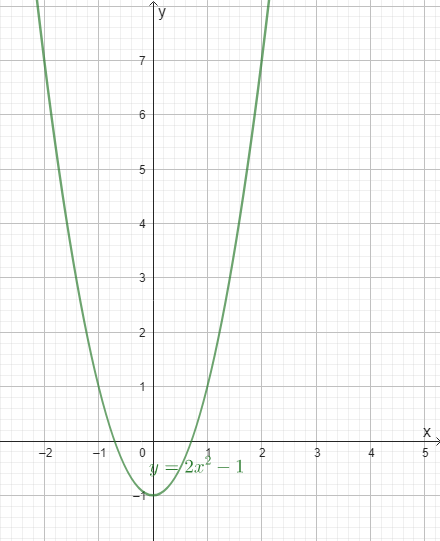
\includegraphics[width=0.35\columnwidth]{figure/1.5q.png}
        \caption{Equation of $y=2x^{2}-1$}
        \label{fig:1.5q}
    \end{figure}
    
    \end{answer}
    
    
    \begin{answer}[Question 1.6]
    \textbf{Collision Detection of Balls}: \\
    For calculating collision, we only care about a ball’s position in space, as well as its size. We can store a ball’s position with the (x, y) coordinates of its center point, and we can calculate its size if we know its radius $r$. Thus, we represent a ball in 2D space as a tuple of (x, y, r). To figure out if two balls are colliding, we need to compute the distance between their centers, then see if this distance is less than or equal to the sum of their radius. If so, they are colliding.
    Please define a function with two list as inputs (two balls' position and radius [x,y,r]), test your function with three different cases.
    \end{answer}
    
    
    \begin{answer}[Question 1.7]
    \textbf{Scoring the words}
    A set of score is given to you as below according to each English letters: 
    LETTER_VALUES = { 'a': 1, 'b': 1, 'c': 5, 'd': 6, 'e': 1, 'f': 4, 'g': 2, 'h': 4, 'i': 1, 'j': 8, 'k': 6, 'l': 1, 'm': 4, 'n': 1, 'o': 1, 'p': 3, 'q': 11, 'r': 1, 's': 1, 't': 1, 'u': 1, 'v': 5, 'w': 4, 'x': 8, 'y': 6, 'z': 10, ' ':100 }\\

    Please finish the ``\texttt{get_word_score}" function for returning the correct word score (condition is given from function comments). The necessary library is given to you for importing (not other libraries should be used). Test with ``Australia", ``Deakin" and your name for three cases.

    \begin{lstlisting}[language=Python]
def get_word_score(word):
    """
    Returns the score for a word. Assumes the word is a
    valid word.

    You may assume that the input word is always either
    a string of letters,
    and can not be the empty string "". 
    You may not assume that the string will only contain
    lowercase letters, so you will have to handle uppercase 
    and mixed case strings
    appropriately.

    The score for a word is the product of two components:

	The first component is the sum of the points for letters 
    in the word.
	The second component is the larger of:
     1, or
     7*wordlen - 3*(20-wordlen),
     where wordlen is the length of the word

    Letters are scored as in LETTER_VALUES.

    word: string
    returns: int >= 0
    """
    \end{lstlisting}
    
    \end{answer}
    
    
    \begin{answer}[Question 1.8]
     Could you please use loop(s) with string character``*" to print as below Figure~\ref{fig:1.8q}?
     \begin{figure}[H]
        \centering
        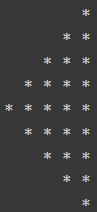
\includegraphics[height=4cm,keepaspectratio]{figure/1.8q.png}
        \caption{Program and Print the shape}
        \label{fig:1.8q}
    \end{figure}
    \end{answer}
    
    \part{Python Foundations for Data Science}\label{sec:part2}

    This part is for students who are aiming to 
    achieve `\texttt{High Distinction}' (HD) for this assessment task. The \Cref{sec:part2} has been designed for a particular scenario based data science problems.

    There are \textbf{2} versions in this part for \textbf{20} marks:
    \textbf{10} marks for coding, \textbf{5} marks for video presentation \texttt{SIT742Task1Part2.avi} 
    (as in~`\textbf{What to Submit}')
    and \textbf{5} marks for the essay \texttt{SIT742Task1Part2report.pdf} (as in~`\textbf{What to Submit}'). 
  
    
    For your question,
    you are required to use \texttt{Google Colab} 
    to finish all the coding in the \textit{code block cell}, 
    provide sufficient coding comments, 
    and also save the result of running.   
    
    \section{Which question for you?}\label{sec-which}

    \begin{lstlisting}

    def sum_digits(n):
        r=0
        while n:
            r, n = r + n % 10, n // 10
        return r

    def check_studentid(studentid):
        x = sum_digits(studentid)
        if x % 2 == 0:
            print ('version I')
        else :
            print ('version II')

    print('Correct Version of Q2 for me is:')
    #check_studentid ()
    \end{lstlisting}

    \section{Question $2$ - Version-I}
    
    \begin{answer}[Question 2: Calculate the Area between a curve and a line]
    
    There are two functions  $y=10-2x$  and  $y=5+4x-x^{2}$ The interaction of the two function is shown as below graph. It could been seen that the area (highlighted with red color) is where the  $y=5+4x-x^{2}$ value larger than  $y=10-2x$ like Figure~\ref{fig:2.1q}. This scenario we could call it as ``Area between a curve and a line". Now your task is to write few functions and draw some graphs to calculate this ``Area between a curve and a line". \\
    \begin{figure}[H]
        \centering
        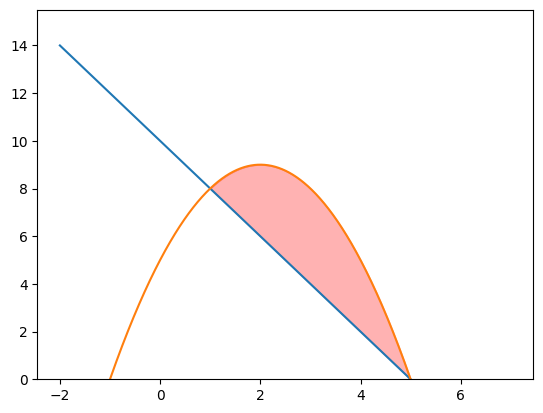
\includegraphics[height=4cm,keepaspectratio]{figure/2.1q.png}
        \caption{The area between $y=10-2x$  and  $y=5+4x-x^{2}$}
        \label{fig:2.1q}
    \end{figure}
    
    
    \textbf{Question 2.1} \\
    The first step is to find out the ``the intersection of the curve and the line" like below graph:
    \begin{figure}[H]
        \centering
        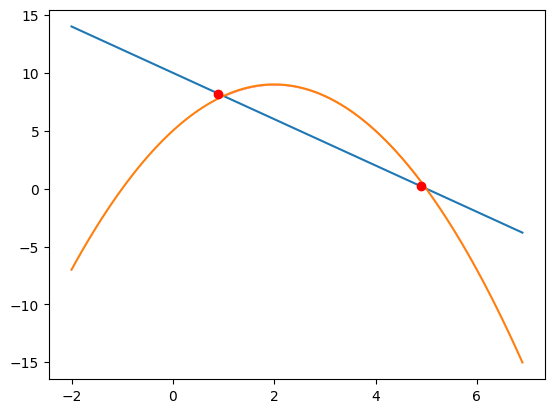
\includegraphics[height=4cm,keepaspectratio]{figure/2.11q.png}
        \caption{The intersection of $y=10-2x$  and  $y=5+4x-x^{2}$}
        \label{fig:2.11q}
    \end{figure}

    Could you please continue working in the graph function to draw ``the intersections of the curve and the line" like Figure~\ref{fig:2.11q}? Also could you print out the two intersections corresponding x and y pair value? 
    (you could round the x and y pair value)

    \begin{lstlisting}
        def graph(formula1,formula2, x_range):
            x = np.array(x_range)
            #use x as range variable
            y1 = formula1(x)
            y2 = formula2(x)
            #call the lambda expression with x on each
            #equation formula, it is given to you 
            #use y1 and y2 as function result
            plt.plot(x,y1)
            plt.plot(x,y2)
            plt.fill_between(x, y1, y2,where=(y1 < y2),
            color='red', alpha=0.3)
            # your code to fill below
            
            plt.ylim(ymin=0)
            plt.show()
            # your code to print the two intersections 
            #x and y pair values in list or tuples [x1,y1] 
            #and [x2,y2]?
            #end of function, no return values
            
        #run the graph function to test your code for marking 
        graph(lambda x : (10 - 2*x), lambda x : (4*x - x**2) +5,
        np.arange(-2, 7, 0.0001))
    \end{lstlisting}
    
    
    \textbf{Question 2.2}
    
    The second step is to find out ``the area under the curve  $y=5+4x-x^{2}$ "by using the two intersections like below Figure~\ref{fig:2.2q}

      \begin{figure}[H]
        \centering
        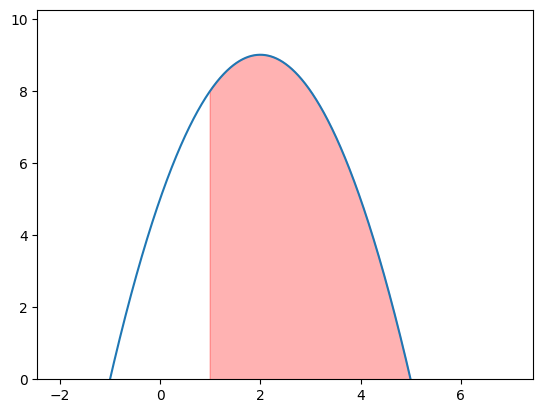
\includegraphics[height=4cm,keepaspectratio]{figure/2.2q.png}
        \caption{The the area under the curve $y=5+4x-x^{2}$}
        \label{fig:2.2q}
    \end{figure}
     You will need to modify the above \texttt{graph} function and draw the graph \textbf{exactly} like Figure~\ref{fig:2.2q}.
     Also you need to finish the code and define the function \texttt{area_curve} and calculate
     the area under the curve $y=5+4x-x^{2}$ with two intersections x and y 
     pair values you obtained in \textbf{Question 2.1}. \\

     \texttt{Hint:} to calculate ``the area under the curve" you need to use \emph{Trapezoidal Rule Formula}. You could find the steps to calculate in \url{https://en.wikipedia.org/wiki/Trapezoidal_rule} \\

     \begin{lstlisting}
         def area_curve(p1,p2):
              """
              your code here, p1 and p2 are [x1,y1] 
              and [x2,y2] pair values
              """
     \end{lstlisting}

     \textbf{Question 2.3} \\
     The third step is to find out ``the area under the line $y=10-2x$" by using the two intersections like below Figure~\ref{fig:2.3q}
    \begin{figure}[H]
        \centering
        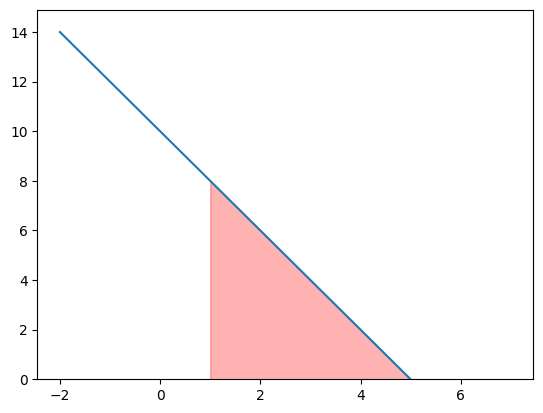
\includegraphics[height=4cm,keepaspectratio]{figure/2.3q.png}
        \caption{The the area under the line $y=10-2x$}
        \label{fig:2.3q}
    \end{figure}

    You will need to modify the above \texttt{graph} function and draw the graph \textbf{exactly} like Figure~\ref{fig:2.3q}.
     Also you need to finish the code and define the function \texttt{area_line} and calculate
     the area under the line $y=10-2x$ with two intersections x and y 
     pair values you obtained in \textbf{Question 2.1}. \\

    \begin{lstlisting}
         def area_line(p1,p2):
              """
              your code here, p1 and p2 are [x1,y1] 
              and [x2,y2] pair values
              """
     \end{lstlisting}

     \textbf{Question 2.4} \\
     The list step is to subtract the two calculated area to obtain the ``area between curve and line" Please run the above defined functions \texttt{area_curve} and \texttt{area_line} to return the value of the area between curve and line (you could round the result to 3 decimals).
    
    \end{answer}

    
    
    \section{Question $2$ - Version-II}
    
    \begin{answer}[Question 2 Buying a House -- how long you need to save for your initial payment?]
    
   You have moved to Melbourne to start your life and decide to get into the property market as soon as possible. The house price is high and you want to save the money for some years (months) before you could afford the down-payment (initial payment) of the house. In this part, we will program to calculate how long you need to save for make the payment of the house. \\

   There are few rules (variables) you need to define to calculate:
   \begin{itemize}
       \item Call the cost of your home \texttt{total_cost}.
       \item Call the portion of the cost needed for a initial payment \texttt{portion_down_payment}. For simplicity, assume that $\texttt{portion_down_payment} = 0.15 (15\%)$.
       \item Call the amount that you have saved so far as  \texttt{current_savings}. You start with a current savings of $0$.
       \item Assume that you invest your current savings wisely, with an annual return of $r$ (in other words, at the end of each month, you receive an additional $\texttt{current_savings}*r/12$ funds to put into your savings – the $r$ is an annual rate). Assume that your investments earn a return of $r = 0.04$.
       \item Assume your annual salary is \texttt{annual_salary}.
       \item Assume you are going to dedicate a certain amount of your salary each month to saving for the down payment. Call that \texttt{portion_saved}. This variable should be in decimal form.
       \item At the end of each month, your savings will be increased by the return on your investment, plus a percentage of your monthly salary ($\texttt{annual_salary} / 12$).
   \end{itemize}




    \textbf{Question 2.1} \\
 
    In this question, your \texttt{annual_salary} is fixed while you are saving for your house initial payment. 
    To finish this question, you need to write a program in python (function or syntax code). Your program should ask user to enter the following variables and return the months you need to save:
    \begin{itemize}
    \item The starting annual salary (\texttt{annual_salary}).
    \item The portion of salary to be saved (\texttt{portion_saved}).
    \item The cost of your dream home (\texttt{total_cost}).
    \end{itemize}

    \textbf{Question 2.2} \\
    
    We unrealistically assumed that your salary did not change. 
    As you are \texttt{Deakin} Master student, clearly you will receive a raise on your salary with time! So we are going to build on your solution to \texttt{question 2.1} by factoring in a raise every $12$ months.\\

    In order to program it with a salary raise, you need to have additional input \texttt{annual_raise} (as a decimal percentage). 
    We will assume your salary will raise every 12 months with your input percentage and calculate how many months it will take you save up enough money for a down payment. Like before, assume that your investments earn a return of $r = 0.04$ (or 4\%) and the required down payment percentage is $0.15$ (or 15\%). Have the user enter the following variables and return the months you need to save \\
    
    \begin{itemize}
        \item The starting annual salary (\texttt{annual_salary}).
        \item The portion of salary to be saved (\texttt{portion_saved}).
        \item The cost of your dream home (\texttt{total_cost}).
        \item The annual salary raise (\texttt{annual_raise}).
    \end{itemize}
           
    \end{answer}
    
    
\end{document}
